% Dielektrikum im Plattenkondensator: ausgerichtete Dipole, gebundene Flächenladungen, geschwächtes Feld
% Gemeinsamer Stil für alle Abbildungen (TikZ -> SVG, siehe figures/build.mjs).
%
% Farben sind Platzhalter ("Sentinels"): build.mjs ersetzt sie im SVG durch
% CSS-Variablen, damit die Abbildungen im hellen und dunklen Modus passen.
% Andere Farben (auch schwarz/weiß) bricht der Build mit Fehler ab.
%
%   fg    Linien, Beschriftung          -> --dark
%   mu    Hilfslinien, Achsen, Maße      -> --gray
%   acc   das eine Konzept der Abbildung -> --secondary (Lime/Oliv)
%   blue  zweite Größe, negative Ladung  -> --fig-blue
%   warm  dritte Größe, positive Ladung  -> --fig-warm
%   bg    Seitenhintergrund (Aussparen)  -> --light
%
% Kein \clip verwenden: pdftocairo macht daraus Clip-Gruppen, in denen exakt
% waagerechte/senkrechte Linien verschwinden. Berechnete Kurven schneidet
% gen/*.py selbst am Rahmen ab.
\documentclass[tikz,border=3pt]{standalone}
\usepackage{amsmath,amssymb,bm}
% Text serifenlos wie die Seite, Mathe in Computer Modern wie KaTeX
\renewcommand{\familydefault}{\sfdefault}
\usetikzlibrary{arrows.meta,calc,decorations.markings,patterns,3d,positioning,angles,quotes}

\definecolor{fg}{RGB}{1,2,3}
\definecolor{mu}{RGB}{4,5,6}
\definecolor{acc}{RGB}{7,8,9}
\definecolor{blue}{RGB}{10,11,12}
\definecolor{warm}{RGB}{13,14,15}
\definecolor{bg}{RGB}{16,17,18}

% Vektoren wie auf der Website (KaTeX \mathbf)
\newcommand{\vv}[1]{\mathbf{#1}}

\tikzset{
  every picture/.style={fg, line width=0.8pt, line cap=round, line join=round,
    >={Stealth[length=5.5pt,width=4.4pt]}},
  every node/.style={font=\small},
  % Linientypen
  main/.style={line width=0.9pt},
  thin/.style={line width=0.5pt},
  aux/.style={mu, line width=0.5pt, dash pattern=on 2.5pt off 2pt},
  axis/.style={mu, line width=0.6pt, ->},
  vec/.style={line width=1.1pt, ->},
  field/.style={line width=0.7pt, postaction={decorate},
    decoration={markings, mark=at position #1 with {\arrow{Stealth[length=4.5pt,width=3.6pt]}}}},
  field/.default=0.5,
  % Flächen
  soft/.style={fill=#1, fill opacity=0.14},
  soft/.default=acc,
  % Ladungen
  qpos/.style={circle, fill=warm, inner sep=0pt, minimum size=9pt,
    path picture={\draw[bg, line width=0.9pt] ($(path picture bounding box.center)+(-2pt,0)$) -- +(4pt,0)
      ($(path picture bounding box.center)+(0,-2pt)$) -- +(0,4pt);}},
  qneg/.style={circle, fill=blue, inner sep=0pt, minimum size=9pt,
    path picture={\draw[bg, line width=0.9pt] ($(path picture bounding box.center)+(-2pt,0)$) -- +(4pt,0);}},
  dot/.style={circle, fill=fg, inner sep=0pt, minimum size=3pt},
  % Beschriftung mit Aussparung, damit Linien den Text nicht kreuzen
  lbl/.style={fill=bg, inner sep=1.5pt},
  % Icons: kräftigere Linien, keine Schrift
  icon/.style={line width=1.6pt, >={Stealth[length=6pt,width=5pt]}},
}

\begin{document}
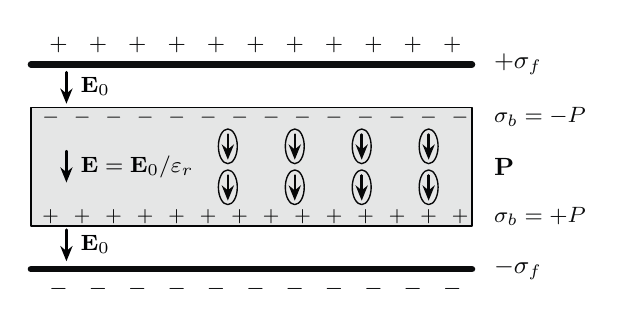
\begin{tikzpicture}
  \def\W{5.6}
  % Platten mit freien Ladungen
  \draw[warm, line width=2.4pt] (0,2.6) -- (\W,2.6);
  \draw[blue, line width=2.4pt] (0,0) -- (\W,0);
  \foreach \x in {0.35,0.85,...,5.4} {
    \node[warm, font=\footnotesize] at (\x,2.85) {$+$};
    \node[blue, font=\footnotesize] at (\x,-0.25) {$-$};
  }
  \node[warm, anchor=west] at (\W+0.15,2.6) {$+\sigma_f$};
  \node[blue, anchor=west] at (\W+0.15,0) {$-\sigma_f$};
  % Dielektrikum
  \fill[mu, fill opacity=0.1] (0,0.55) rectangle (\W,2.05);
  \draw[mu, thin] (0,0.55) rectangle (\W,2.05);
  % Dipole (p parallel zu E, also nach unten): oben negativ, unten positiv
  \foreach \x in {2.5,3.35,4.2,5.05} \foreach \y in {1.04,1.56} {
    \draw[acc, thin] (\x,\y) ellipse (0.12 and 0.22);
    \draw[acc, ->, line width=0.9pt] (\x,\y+0.15) -- (\x,\y-0.17);
  }
  % gebundene Flächenladungen sigma_b = P.n
  \foreach \x in {0.25,0.65,...,5.45} {
    \node[blue, font=\scriptsize] at (\x,1.93) {$-$};
    \node[warm, font=\scriptsize] at (\x,0.67) {$+$};
  }
  % Felder: im Spalt E_0, im Dielektrikum schwächer
  \draw[vec] (0.45,2.5) -- (0.45,2.1);
  \draw[vec] (0.45,0.5) -- (0.45,0.1);
  \node[anchor=west, font=\footnotesize] at (0.5,2.32) {$\vv E_0$};
  \node[anchor=west, font=\footnotesize] at (0.5,0.32) {$\vv E_0$};
  \draw[vec, line width=0.8pt] (0.45,1.5) -- (0.45,1.1);
  \node[anchor=west, font=\footnotesize] at (0.5,1.3) {$\vv E=\vv E_0/\varepsilon_r$};
  % Beschriftung
  \node[acc, anchor=west] at (\W+0.15,1.3) {$\vv P$};
  \node[blue, anchor=west, font=\footnotesize] at (\W+0.15,1.93) {$\sigma_b=-P$};
  \node[warm, anchor=west, font=\footnotesize] at (\W+0.15,0.67) {$\sigma_b=+P$};
\end{tikzpicture}
\end{document}
